\documentclass[journal]{IEEEtran}

\usepackage{tikz}
\usepackage{pgfplots}
\pgfplotsset{compat=1.18}
\usetikzlibrary{arrows.meta,positioning,shapes.geometric,fit,calc,backgrounds}
\usepackage{xcolor}
\usepackage{mdframed}
\usepackage{amsmath,amssymb}
\usepackage{booktabs}
\usepackage{colortbl}
\usepackage{array}
\usepackage{url}
\usepackage{hyperref}

% ---- Rule Q palette (exact values from references/visual-design.md --
% earlier draft used self-invented RGB values; these are the skill's
% documented, tested ones) ----
\definecolor{darkblue}{RGB}{0,0,139}
\definecolor{midgreen}{RGB}{34,139,34}
\definecolor{deepred}{RGB}{180,0,0}
\definecolor{steelblue}{RGB}{52,102,153}
\definecolor{tealcolor}{RGB}{0,110,110}
\definecolor{ambercolor}{RGB}{204,102,0}
\definecolor{slateblue}{RGB}{90,80,160}

% Five-layer figure/table colors reuse the canonical palette above --
% aliases, not new colors, so every existing Fig. 1/2/Table I usage of
% these names now points at the skill's documented values.
\colorlet{promptclr}{tealcolor}
\colorlet{contextclr}{steelblue}
\colorlet{harnessclr}{ambercolor}
\colorlet{agentclr}{slateblue}
\colorlet{loopclr}{deepred}

\hypersetup{colorlinks=true,linkcolor=darkblue,citecolor=darkblue,urlcolor=darkblue}

% Suppress IEEEtran's hardcoded "Abstract---"/"Index Terms---" labels in
% two-column mode so our own colored labels inside the mdframed boxes are
% the only ones that render (references/visual-design.md's documented
% pattern -- \renewcommand{\abstractname}{} alone does not work, the
% "---" is hardcoded in IEEEtran.cls).
\makeatletter
\def\abstract{\normalfont
    \if@twocolumn
      \relax
    \else
      \bgroup\par\addvspace{0.5\baselineskip}\centering\vspace{-1.78ex}%
      \@IEEEabskeysecsize\textbf{\abstractname}%
      \par\addvspace{0.5\baselineskip}\egroup\quotation\@IEEEabskeysecsize
    \fi\@IEEEgobbleleadPARNLSP}
\def\IEEEkeywords{\normalfont
    \if@twocolumn
      \relax
    \else
      \bgroup\par\addvspace{0.5\baselineskip}\centering\@IEEEabskeysecsize%
      \textbf{\IEEEkeywordsname}%
      \par\addvspace{0.5\baselineskip}\egroup\quotation\@IEEEabskeysecsize
    \fi\@IEEEgobbleleadPARNLSP}
\makeatother

\begin{document}

\title{\textcolor{darkblue}{From Prompt Engineering to Loop Engineering: A Five-Layer Taxonomy for Evaluating AI Systems Engineering Practice}}

\author{\IEEEauthorblockN{\textcolor{slateblue}{\itshape Muhammad Faisal Laiq \qquad Email:~shmlaiq@gmail.com \qquad ORCID:~0009-0007-5779-9836}}}

\maketitle

% Standard IEEEtran abstract/keywords environments (Rule Q colored boxes
% nested inside). \IEEEtitleabstractindextext was tried first but silently
% dropped its content under this class configuration on compile -- verified
% by inspecting the rendered PDF, not assumed -- so this is the reliable
% fallback used by essentially every published IEEEtran journal paper.
\begin{abstract}
\begin{mdframed}[
  linecolor=darkblue, linewidth=1.8pt,
  backgroundcolor=darkblue!5,
  innerleftmargin=10pt, innerrightmargin=10pt,
  innertopmargin=9pt, innerbottommargin=9pt,
  roundcorner=5pt, skipabove=0pt, skipbelow=0pt
]
\noindent\textbf{\textcolor{darkblue}{Abstract\,---}}~Large language model (LLM) application development has moved, in roughly five years, from hand-tuning a single input string to operating autonomous systems that plan, call tools, and revise their own output across multiple passes. Practitioners now use ``prompt engineering,'' ``context engineering,'' ``agent engineering,'' and, more recently, ``harness engineering'' and ``loop engineering'' almost interchangeably, even though each term names a distinct engineering discipline with its own failure modes and its own way of measuring success. This paper proposes a five-layer taxonomy---Prompt Engineering, Context Engineering, Harness Engineering, Agent Engineering, and Loop Engineering---that separates these disciplines by what is actually being engineered at each stage: the input string, the surrounding information, the tool-and-permission scaffold, the delegation and planning behavior, and the iterative act-observe-verify cycle, respectively. For each layer we define boundary conditions relative to its neighbors, propose a concrete evaluation metric, and ground the layer in one published system from the literature and one first-person practitioner artifact drawn from an active multi-agent deployment. The paper is a taxonomy and case-study contribution, not a controlled experiment: its claims about the practitioner artifacts are illustrative, not measured, and we say so explicitly rather than let the distinction blur. We argue the taxonomy's principal practical use is diagnostic---identifying which layer a failing AI system is actually missing, particularly the common and under-diagnosed failure of building an agent without a loop, which produces confident but unverified output.
\end{mdframed}
\end{abstract}

\begin{IEEEkeywords}
\begin{mdframed}[
  linecolor=darkblue!35, linewidth=0.8pt,
  backgroundcolor=darkblue!3,
  innerleftmargin=8pt, innerrightmargin=8pt,
  innertopmargin=5pt, innerbottommargin=5pt,
  roundcorner=3pt, skipabove=0pt, skipbelow=4pt
]
\noindent\textbf{\textcolor{darkblue}{Index Terms\,---\,}}prompt engineering, context engineering, autonomous agents, multi-agent systems, software engineering taxonomy, large language models (LLMs)
\end{mdframed}
\end{IEEEkeywords}

\section{\textcolor{darkblue}{Introduction}}

For most of computing history, giving a program intelligence meant writing the rules yourself: a system's behavior was exactly the logic an engineer had hand-coded into it, no more and no less, and improving that intelligence meant improving the code. Large language models broke that equivalence. A model's behavior comes from training, not from any rule a practitioner authored line by line, and the taxonomy this paper proposes exists because the disciplines that once governed hand-coded intelligence do not automatically transfer to a component nobody directly wrote.

Five years ago, getting useful behavior out of a language model meant finding the right words. Today it means operating a system: a model wrapped in retrieval, tools, delegation logic, and a verification loop that decides whether the system's own output is good enough to ship. The vocabulary practitioners use has not kept pace with that shift. A job posting for ``prompt engineer'' and a job posting for ``AI agent engineer'' frequently describe the same work, and a postmortem that concludes ``the prompt needs work'' often turns out, on inspection, to be a missing retrieval step, a tool that fails silently, or an agent that never checks its own answer before returning it.

This is not merely a terminology complaint. Teams that lack a shared vocabulary for \emph{which} discipline is failing tend to apply the wrong fix---rewording a prompt when the real problem is that the model never sees the right context, or adding another layer of agent autonomy when the real problem is that no step in the pipeline ever verifies anything. Vendors selling ``prompt engineering'' courses, ``context engineering'' frameworks, and ``agentic AI'' platforms compound the confusion by using the terms as marketing labels rather than as engineering disciplines with distinct inputs, outputs, and failure signatures.

This paper's contributions are:

\begin{enumerate}
\item A five-layer taxonomy---Prompt Engineering, Context Engineering, Harness Engineering, Agent Engineering, Loop Engineering---that separates what is engineered at each stage of building an LLM-based system, with explicit boundary conditions between adjacent layers.
\item A proposed evaluation metric for each layer, designed to be diagnostic: given a failing system, the metrics are meant to help identify which layer actually needs work.
\item Ten case studies, two per layer---one drawn from the published literature and one a first-person practitioner artifact from an active multi-agent deployment---grounding each layer in something that actually exists rather than only in definition.
\item A discussion of the taxonomy's diagnostic use, including the specific and, we argue, systematically under-diagnosed failure of agent systems that lack any verification loop.
\item A mapping of each layer onto a pre-existing software engineering discipline---Design by Contract, configuration management, containerization, the actor model, and continuous delivery, respectively---that clarifies which difficulties are genuinely new to the LLM era and which are decades-old engineering concerns recurring under new vocabulary.
\end{enumerate}

We are explicit about the shape of this contribution: this is a taxonomy and case-study paper, not a controlled experiment. We did not run a benchmark, recruit participants, or measure the proposed metrics across a sample of systems. Two of the five layers' practitioner case studies (Sections~V-C through V-E) draw on artifacts the first author personally authored; we treat these as existence proofs that the taxonomy's categories are instantiable in real, currently-running practice, not as generalizable evidence that the taxonomy is optimal, and we return to this limitation directly in Section~VII rather than leaving it implicit.

The remainder of this paper proceeds as follows. Section~II reviews the literature underlying each of the five layers. Section~III defines the taxonomy formally, including the boundary conditions between layers. Section~IV proposes an evaluation metric per layer. Section~V presents the ten case studies. Section~VI discusses the taxonomy's practical, diagnostic use. Section~VII states limitations and threats to validity. Section~VIII traces each layer back to a pre-existing software engineering discipline that predates language models entirely. Section~IX concludes with future work ordered by urgency.

\section{\textcolor{darkblue}{Related Work}}

\subsection{\textcolor{darkblue}{Prompt Engineering}}

The modern practice of prompt engineering traces to the observation that large pretrained language models can perform new tasks from a handful of in-context examples without any parameter update---the few-shot learning behavior demonstrated at scale by GPT-3 \cite{brown2020language}. That single finding created an entire discipline: since the model itself is frozen, the only lever available to a practitioner is the string placed in front of it, and a substantial body of technique grew up around how to phrase, order, and exemplify that string. Chain-of-thought prompting \cite{wei2022chain} showed that asking a model to produce intermediate reasoning steps before its final answer measurably changes performance on multi-step reasoning tasks, and follow-up work showed the same effect could be triggered with a simple instruction rather than worked examples \cite{kojima2022large}. What unites this literature is that the model and its weights are treated as fixed; the entire engineering surface is the text of the prompt itself. None of it repairs a missing retrieval step. A rephrased prompt cannot supply information the model was never shown.

The prompt-engineering literature bifurcates into hand-crafted and automatically-searched technique. AutoPrompt \cite{shin2020autoprompt} treats prompt discovery as a gradient-guided discrete search: it computes the gradient of task loss with respect to a one-hot embedding of each trigger-token position, shortlists candidate replacement tokens via a first-order Taylor approximation, and re-scores each candidate by substitution---a formal search procedure, but one that requires white-box gradient access and does not transfer to API-only models. The Automatic Prompt Engineer \cite{zhou2022large} instead treats instruction generation itself as a black-box optimization problem an LLM can solve for another LLM: a proposal model generates candidate instructions from a handful of demonstration pairs, each candidate is scored on held-out task performance, and the best candidates are iteratively refined by resampling variations. APE-discovered prompts outperformed human-written prompts on all 24 instruction-induction tasks tested and improved zero-shot chain-of-thought prompts specifically---direct evidence that the search space Section~V-A's chain-of-thought case study explores by hand can itself be automated.

What counts as a ``good prompt'' is also not fixed across model variants of otherwise-identical weights. Instruction tuning \cite{wei2021finetuned} finetunes a base model on tens of task categories rewritten into multiple natural-language instruction templates, then evaluates zero-shot on entirely unseen categories; reinforcement learning from human feedback \cite{ouyang2022training} goes further, training a reward model on human rankings of candidate outputs and optimizing the policy against that reward via PPO, a process that improved instruction-following, honesty, and toxicity simultaneously rather than only task-format compliance. Both processes change the frozen weights a prompt is written against, meaning a fixed prompt engineered for a base model is not guaranteed to transfer to an instruction-tuned or RLHF'd variant of the same underlying model---a second, independent way this layer's boundary is porous, distinct from its boundary with Layer 2.

Two findings ground the mechanistic and empirical basis of few-shot prompting itself. Induction heads \cite{olsson2022incontext}---a two-attention-head circuit that performs prefix-matching and copies the matched continuation into the output---form during a sharp phase transition in training that coincides with in-context learning ability improving sharply, the closest mechanistic, not merely behavioral, account of why a demonstration in the prompt changes model output at all. Earlier still, well-designed zero-shot prompts were shown to outperform few-shot prompts on the same task \cite{reynolds2021prompt}, suggesting few-shot examples often function to locate a capability already present from pretraining rather than to teach a new one---an early articulation of exactly this layer's definition, predating the term ``prompt engineering'' itself. A systematic survey \cite{liu2021pretrain} formalized ``prompt-based learning'' as a paradigm shift from pretrain-then-finetune, decomposing the design space by prompt shape (cloze vs.\ prefix) and by hand-crafted vs.\ automatically-searched vs.\ continuous or soft prompts---a finer-grained taxonomic effort within what this paper treats as a single layer.

Self-consistency \cite{wang2022selfconsistency} sits at this layer's upper boundary. Rather than a single greedy chain-of-thought decode, it samples a diverse set of reasoning paths at non-zero temperature and returns the answer with the most votes among them, reporting a 17.9-point gain on GSM8K over greedy decoding. By this paper's own Section~III definition, majority-voting across a model's own samples is a self-consistency check, not an externally-verified one; it belongs conceptually closer to Layer~1's prompt-and-sample technique than to Layer~5's external-verifier requirement, and we flag that boundary explicitly here rather than let it blur unstated.

\subsection{\textcolor{darkblue}{Context Engineering}}

Prompt engineering hits a hard ceiling the moment a task requires information the model was never trained on, or information that changes after training---a live database, a private document set, today's date. Retrieval-Augmented Generation \cite{lewis2020retrieval} addressed this by pairing a frozen or fine-tuned generator with a retriever that pulls relevant passages into the model's input at inference time, moving the engineering problem from ``what do I say'' to ``what does the model need to see.'' Anthropic's own practitioner guidance names this discipline directly, defining context engineering as curating and maintaining the optimal set of tokens available to the model at inference time and treating context as a limited resource to be spent deliberately rather than filled by default \cite{anthropic2025context}. We use ``context engineering'' as the broader successor discipline to retrieval alone: the curation of everything that surrounds the instruction in the context window---conversation history, tool outputs, memory records, system instructions---and the decisions about what to include, what to omit, and how to order it so the model reasons over the right material. Context engineering treats the prompt's wording as secondary to the information assembled around it. That curation problem is not academic: models given long, retrieval-heavy contexts do not use every part of them equally, showing markedly worse recall for information placed in the middle of the context window than for information at either end \cite{liu2023lost}, and a recent survey of production RAG systems catalogs the resulting engineering practice---chunking, re-ranking, and query rewriting---as responses to exactly that failure pattern \cite{gao2023retrieval}. Retrieval is not comprehension. A passage sitting in the context window does not mean the model actually used it.

The retrieval mechanism RAG depends on is itself an active engineering surface. Dense Passage Retrieval \cite{karpukhin2020dense} replaced sparse lexical matching---BM25 and TF-IDF term overlap---with a dual-encoder architecture: separate BERT encoders embed the query and each candidate passage, and retrieval becomes nearest-neighbor search in the shared embedding space, reporting 9--19 absolute points of top-20 accuracy over BM25 and supplying the retriever the paper's already-cited RAG mechanism is built on top of. ColBERT \cite{khattab2020colbert} occupies a documented middle ground between DPR's fast-but-shallow bi-encoders and slow-but-accurate cross-encoders: it encodes query and passage into per-token vectors rather than one vector each, then scores relevance via a MaxSim operator that finds each query token's most similar passage token and sums those maxima, preserving token-level matching precision at roughly two orders of magnitude faster inference than cross-encoders. Retrieval quality is therefore a genuine speed/precision/index-size trade-off space, not a solved primitive this layer can treat as a black box.

Retrieval timing and self-assessment form a second axis of active engineering. Self-RAG \cite{asai2023selfrag} trains a model to emit special reflection tokens that decide, inline with normal generation, whether retrieval is needed for the current segment, whether a retrieved passage is relevant, and whether the generated text is actually supported by that passage---making retrieval adaptive rather than a single fixed pass, and making the resulting judgment inspectable rather than a hidden gate. Corrective RAG \cite{yan2024corrective} instead inserts a lightweight evaluator between retrieval and generation that scores each retrieved document into a correct, ambiguous, or incorrect confidence band and triggers a different remedy per band---refining correct-but-noisy documents, falling back to web search for incorrect ones---a direct, citable answer to what a system should do once Section~V-B's claim that ``the retriever returned the wrong passage'' is diagnosed. FLARE \cite{jiang2023active} takes a third position: rather than retrieving on a fixed schedule, it generates a tentative next sentence, checks that draft's token-level confidence, and only retrieves, using the low-confidence sentence itself as the query, when confidence falls below a threshold---making retrieval timing a continuous decision driven by the model's own uncertainty rather than a trained relevance classifier. We flag directly that Self-RAG's relevance and support checks are themselves self-assessment, not external verification, another instance of this taxonomy's recurring distinction surfacing inside the retrieval pipeline rather than only at the final output.

Context is also a resource to be spent deliberately, not merely retrieved. LLMLingua \cite{jiang2023llmlingua} scores each token's contribution to prompt perplexity using a small auxiliary model, on the premise that low-perplexity tokens carry little information the larger target model needs, then allocates a compression budget across the prompt's instruction, few-shot, retrieved-context, and question components and removes low-information tokens iteratively---reporting up to 20x compression with minimal task-performance loss, and operationalizing ``what to include, what to omit'' as an actual algorithm rather than only a design principle. MemGPT \cite{packer2023memgpt} borrows operating-system virtual memory paging directly: the model's context window is fast ``main memory,'' an external store holds a much larger ``disk'' tier, and the model issues its own tool calls to page content in and out, with self-generated interrupts pausing generation mid-conversation to perform a memory operation. This is a genuine boundary case for the taxonomy: MemGPT's paging decisions are context-layer content selection, but they are executed through tool calls, a Layer~3 mechanism---an instance where the layers compose rather than cleanly separate, which we take as supporting rather than undermining Section~VII's claim that layer boundaries are not always sharp.

Finally, a model's advertised context window and its effective usable context are measurably different quantities. Beyond the single-fact ``needle in a haystack'' test, RULER \cite{hsieh2024ruler} adds multi-needle variants, multi-hop tracing across retrieved locations, and aggregation tasks requiring information combined from many places; evaluating 17 models advertising 32K-plus token windows, only about half maintain acceptable performance at the length they claim to support, with degradation sharpening at longer lengths and higher task complexity. This supplies the multi-model, multi-task empirical scope that this paper's earlier, narrower citation of the same phenomenon \cite{liu2023lost} does not by itself provide.

\subsection{\textcolor{darkblue}{Harness Engineering}}

A model that can only read context and emit text cannot act on the world. Toolformer demonstrated that a language model could learn, largely on its own, when and how to invoke external tools (a calculator, a search API, a calendar) and incorporate their results into its output \cite{schick2023toolformer}. A broader survey of this line of work catalogs the surrounding design space---how a model decides which tool to call, how it formats the call, and how it incorporates the result---as ``tool learning,'' a discipline distinct from the harness that executes the call safely once selected \cite{qin2023tool}. Tool-use and function-calling capability subsequently became a standard feature of production model APIs, and a substantial body of open-source and commercial ``agent framework'' tooling grew up around the scaffolding needed to execute a tool call safely---sandboxing, permissioning, retry logic, error surfacing back to the model. The Model Context Protocol formalized one version of this scaffolding as an open, client-server standard: rather than a bespoke integration per tool, a model-driven application connects through a single protocol to external data sources, tools, and predefined workflows exposed by independent servers \cite{anthropic2024mcp}. Its adoption across multiple independent AI vendors and developer tools, not just its originating company, is itself evidence that the harness layer is a real, separately-engineered concern rather than an artifact of any one vendor's implementation. We adopt the term ``harness engineering'' for this scaffolding layer; unlike the other four layers, this term's academic footing is recent rather than established: Lin et al.'s 2026 study of automatic coding-agent harness evolution is, to our knowledge, the first paper to place ``agentic harness engineering'' in its own title, and industry practitioners had already converged on a compact one-line formulation of the same idea---``Agent = Model + Harness''---in the same period \cite{lin2026agentic,trivedy2026anatomy}. We treat the term as an emerging one with academic usage only as recent as 2026, not as a decades-old settled category the way ``prompt engineering'' now is, and Section~III's boundary conditions are this paper's own contribution to sharpening it rather than a restatement of prior consensus. A safe tool call is not a correct plan. Sandboxing a mistake still ships the mistake.

Concrete implementations of this scaffolding diverge on how tightly the action space is constrained. Gorilla \cite{patil2023gorilla} fine-tunes a model to generate accurate API calls against a retrieval-augmented index of API documentation, addressing two specific failure modes---imprecise argument generation and outright API hallucination---and updating what the model can call without retraining by updating the retrieved documentation instead. ToolLLM \cite{qin2023toolllm} constructs an instruction-tuning corpus of tool-use trajectories across more than 16,000 real-world APIs and introduces a depth-first-search decision tree that lets a model evaluate multiple candidate tool-selection paths rather than committing to one greedy chain, a direct answer to how a harness should structure search over a large tool registry. API-Bank \cite{li2023apibank} decomposes ``can the model use a tool'' into three separately-measured sub-capabilities---planning, retrieval, and invocation---and finds these do not move together across models (GPT-4 stronger at planning, GPT-3.5 at raw invocation), evidence that a harness's tool-registry concern is not a single monolithic capability but several distinct ones. At the more permissive end, CodeAct \cite{wang2024codeact} replaces JSON-schema tool calls with executable Python code as the agent's unified action space, executed inside a Python interpreter---more expressive, since it supports dynamic composition and multi-turn state via variables, but it moves the harness's sandboxing and permission stakes considerably higher, reporting up to 20\% higher task success across 17 models than JSON-style calling specifically because of that expressiveness. ToolkenGPT \cite{hao2023toolkengpt} answers a narrower registry-scaling question directly: representing each tool as a learned-embedding ``toolken'' token lets a frozen model invoke a new tool the same way it emits an ordinary vocabulary token, so the tool registry can grow without retraining the base model at all.

Orchestration is a distinct harness concern from execution. HuggingGPT \cite{shen2023hugginggpt} uses an LLM purely as a controller that decomposes a request into subtasks, selects a specialist model for each from a registry of model descriptions, sequences execution, and synthesizes results---keeping the harness's dispatch role structurally separate from generation. Chameleon \cite{lu2023chameleon} and RestGPT \cite{song2023restgpt} solve an architecturally similar composition problem by different means: Chameleon's planner assembles plug-and-play tool modules via constraint inference over what each module produces and consumes, while RestGPT splits task decomposition from a dedicated executor module that handles REST call formatting and response parsing specifically---the same agent/harness split this paper's Section~III draws, arrived at independently. That there are at least three non-identical architectural answers to essentially the same orchestration problem is itself evidence the harness layer is a real, unsettled design space rather than a solved primitive with one canonical implementation.

The permission and error-formatting half of this layer is not academic. Indirect prompt injection \cite{greshake2023injection} demonstrates that malicious instructions embedded in content a tool-using model merely retrieves---not the user's direct prompt---can hijack the application: triggering unintended API calls, executing arbitrary code, and exfiltrating data, because the model cannot reliably distinguish data it is processing from instructions it should obey. The demonstration is not hypothetical; it was validated against real deployments including Bing Chat. This is the paper's clearest evidence that Layer~3's permission-system and error-formatting concerns exist because harnesses fail concretely when that boundary is porous, not merely because a taxonomy asserts the concern in the abstract.

\subsection{\textcolor{darkblue}{Agent Engineering}}

Once a model has tools and a harness to execute them safely, a further question arises: which tool, in what order, and when should the process stop and ask a human? Anthropic's practitioner-oriented survey ``Building Effective Agents'' \cite{anthropic2024building} draws a widely-cited distinction between \emph{workflows}, in which the control flow is predefined by the engineer, and \emph{agents}, in which the model itself directs its own process and tool use to accomplish a task. Open-source frameworks such as AutoGPT popularized the idea of a single model looping over its own plan with minimal human oversight, while multi-agent frameworks including AutoGen \cite{wu2023autogen} and CrewAI formalized patterns for multiple specialized agents collaborating, delegating subtasks, and communicating results. Generative Agents demonstrated a related but distinct point: giving a population of language-model-driven agents persistent memory, reflection, and planning was enough to produce believable emergent social behavior in a simulated environment, without any of the agents being told what to do turn by turn \cite{park2023generative}. A broader survey organizes this literature around a common brain-perception-action framework spanning single-agent, multi-agent, and human-agent settings \cite{xi2023rise}. This literature is concerned with \emph{decision-making behavior}---planning, task decomposition, delegation, escalation---layered on top of a harness that already exists. None of these frameworks verify their own output. Delegation is not correctness.

Concrete systems instantiate the workflow/agent distinction differently. Voyager \cite{wang2023voyager} combines an automatic curriculum that proposes the next exploration goal to maximize learning progress with an expandable skill library that stores executable code for previously-learned behaviors, so capability accumulates and is reused rather than relearned each session---a code-level answer to how an agent's task-decomposition capability grows over a long-running deployment, directly relevant to this layer's persona-and-voice and delegation concerns. CAMEL \cite{li2023camel} predates AutoGen's role-specialization pattern with ``inception prompting'': two agents are assigned complementary roles and converse autonomously toward task completion with no further human guidance, establishing role-specialized delegation's provenance earlier than the framework this paper already cites. Multiagent debate \cite{du2023debate} takes the opposite structural approach---multiple instances of the identical model each propose an answer, observe each other's reasoning over several rounds, and revise their own position before a final convergent answer, an adversarial-collaborative delegation pattern rather than a role-specialized one, and a black-box wrapper compatible with any existing model.

Two frameworks build agent-to-agent verification directly into the delegation structure. MetaGPT \cite{hong2023metagpt} encodes standardized operating procedures mimicking a real software team---product manager, architect, engineer, QA---with each role explicitly verifying the previous role's output before passing work downstream, motivated directly by cascading hallucination across multi-agent handoffs. ChatDev \cite{qian2023chatdev} solves an architecturally distinct version of the same problem: a ``chat chain'' constrains what agents may communicate about at each development phase, paired with a ``communicative dehallucination'' technique that regulates inter-agent claims specifically to reduce fabrication passed downstream. Both sit exactly on this paper's Agent/Loop boundary---inter-role verification is a delegation-structure decision (Agent Engineering) that happens to also check individual outputs (Loop Engineering's concern)---and we treat their existence as evidence the boundary is a real design tension practitioners have already had to resolve, not an artifact of this paper's own categorization scheme.

Agent-layer capability is also measurably immature relative to prompt and context engineering. AgentBench \cite{liu2023agentbench} evaluates models across eight distinct interactive environments under realistic multi-step conditions and finds a large capability gap between top commercial and open-source models under 70B parameters, attributed specifically to poor long-term reasoning, decision-making, and instruction-following---an agent-layer deficit, not a raw language-modeling one. WebArena \cite{zhou2023webarena} supplies a concrete number for how large that gap can be in a realistic setting: GPT-4-based agents reach 14.41\% task success on real, self-hosted websites against 78.24\% human success on the same tasks. AgentVerse \cite{chen2023agentverse} studies group composition as a first-class variable rather than fixing it at the start of a task, and separately measures emergent social dynamics---both beneficial and counterproductive---among agents, work closer to what Section~IV's delegation-correctness-versus-expert-decomposition metric would need to actually operationalize than a framework that treats group structure as a static design choice. Language Agent Tree Search \cite{zhou2023lats} sharpens the Agent/Loop boundary further still, combining Monte Carlo Tree Search with LLM value functions and self-reflection to search over candidate action sequences using environmental feedback to guide which branches to expand---structurally close to Tree of Thoughts but applied to tool-using action selection rather than pure reasoning, blending planning search (an Agent-layer concern) with outcome-based pruning (a Loop-adjacent one) in a single system.

\subsection{\textcolor{darkblue}{Loop Engineering}}

A system that plans and delegates still has no guarantee that any individual step's output is correct, and asking the model itself whether it is done is a weak check, since the same model that produced an error is often the one asked to certify it. ReAct interleaved reasoning traces with actions and their observed results, letting the model's next reasoning step be grounded in what actually happened rather than what it expected to happen \cite{yao2022react}. Self-Refine showed that a model critiquing and rewriting its own output in successive passes, with no additional training and no external verifier at all, still produced measurable quality gains on a range of tasks---a useful contrast case for this layer, since it is closer to a loop's outer shape than to a loop's substance by our definition, precisely because the check being applied is the model's own judgment rather than anything external to it \cite{madaan2023selfrefine}. Reflexion extended this with an explicit self-critique step: on failure, the agent generates a verbal reflection on what went wrong and carries that reflection into its next attempt, functioning as a linguistic form of reinforcement learning without any weight update \cite{shinn2023reflexion}. Tree of Thoughts generalized single-path reasoning into a search over multiple candidate reasoning paths, evaluated and pruned before a final answer is selected \cite{yao2023tree}. What these three lines of work share, and what we treat as the defining property of this layer, is a mechanical decide-to-continue step: the loop does not simply run once and stop, it observes a real result, checks it against something external to the model's own confidence, and only then decides whether to act again. A self-critique is not an external check. The same model that erred is still the one grading itself.

The central claim of this layer is no longer only a design position; it is a measured empirical result. Huang et al.\ \cite{huang2023large} report directly that large language models struggle to self-correct their own reasoning without external feedback, and that performance at times degrades after self-correction---not merely fails to improve, actively worsens. Kamoi et al.'s survey \cite{kamoi2024can} confirms this is not an isolated finding: across the self-correction literature, no prior work demonstrates successful self-correction using only feedback a model generates about itself, outside narrow task types unusually suited to it, and many earlier ``self-correction works'' results rest on inflated or loose evaluation methodology. Together these two sources convert what this paper states as design intuition---a self-critique is not an external check---into the field's converging empirical consensus rather than one paper's assertion.

Verification mechanisms in the literature differ in exactly how external their check actually is. Self-consistency \cite{wang2022selfconsistency}---already discussed in Section~II-A as a prompt-layer boundary case---samples multiple reasoning paths and votes on agreement, a weaker mechanism than an externally-grounded check since consensus among a model's own samples is still self-assessment, just aggregated rather than singular. Process reward models \cite{lightman2023lets} occupy a genuine middle case: a separate model is trained on human step-level annotations to score each intermediate reasoning step rather than only the final answer, and process supervision significantly outperforms outcome-only supervision on the MATH benchmark---an external check, since the verifier is a distinct trained model, but a probabilistic rather than symbolic one. Constitutional AI \cite{bai2022constitutional} scopes the critique step against an external, written, fixed set of principles rather than the model's own free-floating judgment, generating self-critiques and revisions against that constitution in a supervised phase before training a preference model from AI-generated, not human-generated, judgments for an RL phase---a middle ground between the self-assessment Huang and Kamoi show fails and a fully external deterministic check. CRITIC \cite{gou2023critic} generalizes tool use explicitly into the verification role: the model generates an initial response, then invokes external tools specifically to validate or critique that response before revising---the tools function here as the external check itself, not merely as Section~II-C's execution capability, a direct bridge between the harness and loop layers.

The cleanest and least ambiguous case is a fully symbolic, deterministic verifier. AlphaCode \cite{li2022competitionlevel} generates a large pool of candidate solutions to a competitive-programming problem, runs each against test cases, and submits only survivors---pass/fail against a test suite admits no interpretation, and the system achieved an average top-54.3\% ranking against fields of 5,000-plus Codeforces participants using exactly this filter. STaR \cite{zelikman2022star} shows the same verifier-first principle applies to training as well as inference: an iterative bootstrap generates a rationale for each training question, keeps rationales that led to a correct final answer, regenerates, given the correct answer as a hint, for those that did not, and finetunes only on the rationales that survived that correctness filter---the same deterministic external check this paper's Section~IV argues for at inference time, applied instead to what gets trained on.

An external verifier is also not automatically trustworthy simply because it is external. Scaling laws for reward-model overoptimization \cite{gao2022scaling} show that even a trained proxy verifier can be gamed: optimizing against it via reinforcement learning or best-of-n sampling improves true reward only up to a point before degrading, a Goodhart's-Law failure mode, though larger reward models resist it more than smaller ones. The lineage from Christiano et al.'s original reward-modeling-from-preferences work \cite{christiano2017deep} through InstructGPT's reward-model-plus-PPO pipeline \cite{ouyang2022training} and WebGPT's citation-grounded, human-feedback-trained browsing agent \cite{nakano2021webgpt} establishes that a verifier can itself be a trained model rather than only a symbolic rule---useful nuance for Section~IV's evaluation framework, but one that inherits the same overoptimization caution rather than escaping it. AI Safety via Debate \cite{irving2018ai} supplies a structurally distinct verification pattern entirely: two agents argue opposing positions across alternating turns and a judge, human or in principle another model, decides which was more truthful, extending what a judge can verify from direct judgment to debate-assisted judgment under optimal play. We include it to note explicitly that ``external check'' need not mean a symbolic test; adversarial cross-examination counts too, provided the judge is not the same agent being checked, which is the one condition every mechanism surveyed in this subsection ultimately has to satisfy.

\section{\textcolor{darkblue}{The Five-Layer Taxonomy}}

Each layer answers a different question about what is actually being engineered. The layers are cumulative in the sense that a system operating at Layer~5 still depends on Layers~1 through~4 functioning correctly underneath it---a well-verified loop cannot repair a harness that silently drops half its tool calls, any more than a beautifully worded prompt can repair a retrieval step that returns the wrong document. Fig.~\ref{fig:stack} depicts the stack.

\textbf{Layer 1---Prompt Engineering.} Unit of engineering: the input string. The practitioner treats the model and everything around it as fixed and asks only ``how do I phrase this instruction, and which examples do I show, so that a single forward pass produces the output I want.'' \emph{Boundary with Layer 2:} the moment the practitioner stops asking ``how do I phrase this'' and starts asking ``what information does the model need that simply is not in the prompt yet,'' they have left Layer~1.

\textbf{Layer 2---Context Engineering.} Unit of engineering: the assembled context window---retrieved passages, tool outputs already collected, conversation history, memory records, system instructions---and the policy for what enters it, what is dropped, and in what order. \emph{Boundary with Layer 3:} context engineering answers ``what does the model see''; the moment the question becomes ``what is the model allowed to \emph{do}, and how is that action executed and checked,'' the practitioner has crossed into harness territory.

\textbf{Layer 3---Harness Engineering.} Unit of engineering: the scaffolding that determines what actions a model-driven process may take, how those actions are executed, sandboxed, retried on failure, and reported back to the model---independent of what task is being asked of the model at any given moment. Industry usage has converged on a compact one-line version of this same boundary: ``Agent = Model + Harness'' \cite{trivedy2026anatomy}. A permission system, a tool registry, a retry policy, and an error-formatting convention all live here---MCP servers are a concrete, standardized instance of exactly this registry-and-permission layer, not a competing concept. \emph{Boundary with Layer 4:} harness engineering is infrastructure that exists whether or not anyone is currently using it; the moment engineering effort shifts to \emph{which} tool the system should choose, in what order, and whether to delegate a subtask to another process, that is a decision-making concern, and belongs to the next layer up.

\textbf{Layer 4---Agent Engineering.} Unit of engineering: the decision-making behavior of an autonomous process built atop a harness---task decomposition, tool selection, delegation to sub-agents, persona and voice, and the explicit boundary of what the process may decide unsupervised versus what requires a human. \emph{Boundary with Layer 5:} agent engineering specifies \emph{what the system should decide to do}; it does not, by itself, guarantee that any individual decision or output was actually correct. The moment a mechanism is added whose job is to check a result against something external to the agent's own stated confidence---and to decide, based on that check, whether to try again---the system has entered loop-engineering territory.

\textbf{Layer 5---Loop Engineering.} Unit of engineering: the iterative act-observe-verify-decide cycle that governs whether an agent's own output gets checked, and how it gets revised, before it is accepted as final. The load-bearing property of this layer is a rule we adopt directly from ReAct- and Reflexion-style designs and from practitioner loop-engineering guidance we reviewed while preparing this paper: trust a deterministic, external check, never the agent's own report that it ``looks done.'' A loop without such a check is, by our definition, not actually a loop---it is a chain that happens to run more than once.

No amount of engineering effort at a higher layer compensates for a defect at a lower one. A harness that silently swallows a tool's error message will produce confidently wrong agent decisions no matter how well the agent layer is designed, and a loop's verifier is only as good as the harness-level signal it has to check against.

\begin{figure}[t]
\centering
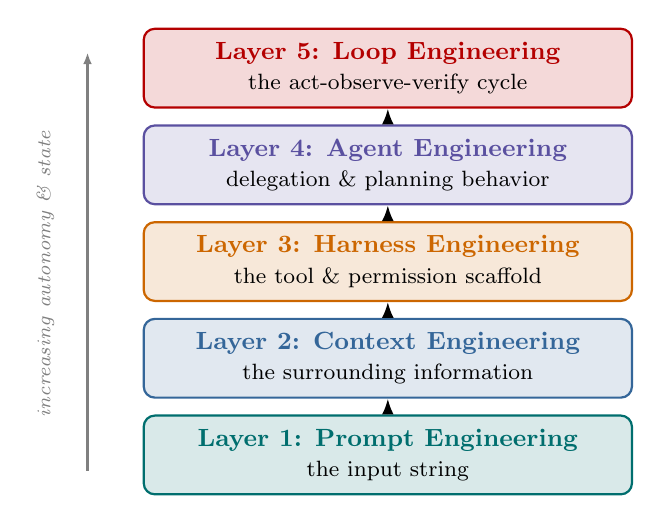
\begin{tikzpicture}[node distance=0.2cm, every node/.style={font=\small}]
  \node[draw=promptclr, fill=promptclr!15, thick, rounded corners, minimum width=6.2cm, minimum height=1cm, align=center] (prompt) at (0,0) {\textbf{\textcolor{promptclr}{Layer 1: Prompt Engineering}}\\ \footnotesize the input string};
  \node[draw=contextclr, fill=contextclr!15, thick, rounded corners, minimum width=6.2cm, minimum height=1cm, align=center, above=of prompt] (context) {\textbf{\textcolor{contextclr}{Layer 2: Context Engineering}}\\ \footnotesize the surrounding information};
  \node[draw=harnessclr, fill=harnessclr!15, thick, rounded corners, minimum width=6.2cm, minimum height=1cm, align=center, above=of context] (harness) {\textbf{\textcolor{harnessclr}{Layer 3: Harness Engineering}}\\ \footnotesize the tool \& permission scaffold};
  \node[draw=agentclr, fill=agentclr!15, thick, rounded corners, minimum width=6.2cm, minimum height=1cm, align=center, above=of harness] (agent) {\textbf{\textcolor{agentclr}{Layer 4: Agent Engineering}}\\ \footnotesize delegation \& planning behavior};
  \node[draw=loopclr, fill=loopclr!15, thick, rounded corners, minimum width=6.2cm, minimum height=1cm, align=center, above=of agent] (loop) {\textbf{\textcolor{loopclr}{Layer 5: Loop Engineering}}\\ \footnotesize the act-observe-verify cycle};

  \draw[-{Latex[length=2mm]}, thick] (prompt.north) -- (context.south);
  \draw[-{Latex[length=2mm]}, thick] (context.north) -- (harness.south);
  \draw[-{Latex[length=2mm]}, thick] (harness.north) -- (agent.south);
  \draw[-{Latex[length=2mm]}, thick] (agent.north) -- (loop.south);

  \node[rotate=90, anchor=south, font=\scriptsize\itshape, gray] at ($(prompt.west)+(-1.0,2.3)$) {increasing autonomy \& state};
  \draw[-{Latex[length=1.5mm]}, gray, thick] ($(prompt.west)+(-0.7,-0.2)$) -- ($(loop.west)+(-0.7,0.2)$);
\end{tikzpicture}
\caption{The five-layer taxonomy, ordered by what is being engineered at each stage. Each layer subsumes the concerns of the layers below it; a defect at a lower layer cannot be repaired by better engineering at a higher one.}
\label{fig:stack}
\end{figure}

\section{\textcolor{darkblue}{Evaluation Framework}}

A taxonomy is only useful in practice if it comes with a way to tell, from the outside, which layer is actually broken. We propose one diagnostic metric per layer, summarized in Table~\ref{tab:metrics} and Fig.~\ref{fig:eval}. Each is designed to isolate a failure at its own layer from a failure at a neighboring one, since misdiagnosis---treating a context problem as a prompt problem, or an agent problem as a loop problem---wastes engineering effort at the wrong point in the stack.

\begin{table}[t]
\centering
\caption{Per-layer diagnostic metrics.}
\label{tab:metrics}
\begin{tabular}{@{}p{1.5cm}p{2.6cm}p{3.5cm}@{}}
\toprule
\rowcolor{darkblue!15}
\textbf{Layer} & \textbf{Metric} & \textbf{Failure signature} \\
\midrule
\rowcolor{promptclr!8}
Prompt & output variance across $k$ equivalent rephrasings & correct on some phrasings, wrong on others, same information available \\
\rowcolor{contextclr!8}
Context & retrieval precision/recall + context-window utilization & confident answer built on content never actually retrieved \\
\rowcolor{harnessclr!8}
Harness & tool-call success rate; error-recovery rate & a tool fails and the agent proceeds as if it succeeded \\
\rowcolor{agentclr!8}
Agent & delegation correctness vs.\ expert decomposition & right tools exist, but work is routed to the wrong step \\
\rowcolor{loopclr!8}
Loop & convergence rate; iterations-to-verified-success & success reported without the verifier ever running \\
\bottomrule
\end{tabular}
\end{table}

The loop-layer metric deserves its own emphasis, because it is where the taxonomy's central diagnostic claim lives: a loop is only as trustworthy as its verifier, and a verifier is only trustworthy if it is deterministic and external to the agent's own self-assessment. Per the layered-termination framing we adopt from loop-engineering practice, a robust loop needs more than one exit condition---a deterministic verifier for the primary pass/fail judgment, plus at least one safety exit such as a hard iteration cap, a budget guard on total tool calls or tokens spent, and no-progress detection that halts a loop whose recent passes changed nothing. A loop that has only a single exit---``stop when the model says it's done''---is not measuring convergence at all; it is measuring the model's own confidence, which is exactly the signal Reflexion-style designs treat as insufficient on its own.

\begin{figure*}[t]
\centering
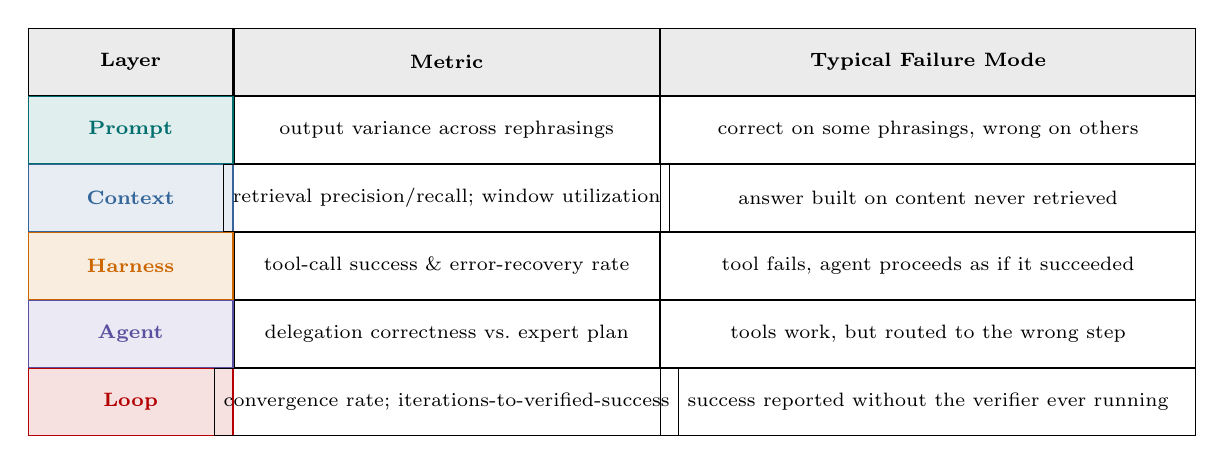
\begin{tikzpicture}[font=\scriptsize, node distance=0.05cm]
  \def\rowh{0.85cm}
  \def\colaw{2.6cm}
  \def\colbw{5.4cm}
  \def\colcw{6.8cm}

  \node[draw, fill=black!8, minimum width=\colaw, minimum height=\rowh, align=center, font=\bfseries\scriptsize] (h1) at (0,0) {Layer};
  \node[draw, fill=black!8, minimum width=\colbw, minimum height=\rowh, align=center, font=\bfseries\scriptsize, right=0cm of h1] (h2) {Metric};
  \node[draw, fill=black!8, minimum width=\colcw, minimum height=\rowh, align=center, font=\bfseries\scriptsize, right=0cm of h2] (h3) {Typical Failure Mode};

  \node[draw=promptclr, fill=promptclr!12, minimum width=\colaw, minimum height=\rowh, align=center, below=0cm of h1] (r1a) {\textcolor{promptclr}{\textbf{Prompt}}};
  \node[draw, minimum width=\colbw, minimum height=\rowh, align=center, below=0cm of h2] (r1b) {output variance across rephrasings};
  \node[draw, minimum width=\colcw, minimum height=\rowh, align=center, below=0cm of h3] (r1c) {correct on some phrasings, wrong on others};

  \node[draw=contextclr, fill=contextclr!12, minimum width=\colaw, minimum height=\rowh, align=center, below=0cm of r1a] (r2a) {\textcolor{contextclr}{\textbf{Context}}};
  \node[draw, minimum width=\colbw, minimum height=\rowh, align=center, below=0cm of r1b] (r2b) {retrieval precision/recall; window utilization};
  \node[draw, minimum width=\colcw, minimum height=\rowh, align=center, below=0cm of r1c] (r2c) {answer built on content never retrieved};

  \node[draw=harnessclr, fill=harnessclr!12, minimum width=\colaw, minimum height=\rowh, align=center, below=0cm of r2a] (r3a) {\textcolor{harnessclr}{\textbf{Harness}}};
  \node[draw, minimum width=\colbw, minimum height=\rowh, align=center, below=0cm of r2b] (r3b) {tool-call success \& error-recovery rate};
  \node[draw, minimum width=\colcw, minimum height=\rowh, align=center, below=0cm of r2c] (r3c) {tool fails, agent proceeds as if it succeeded};

  \node[draw=agentclr, fill=agentclr!12, minimum width=\colaw, minimum height=\rowh, align=center, below=0cm of r3a] (r4a) {\textcolor{agentclr}{\textbf{Agent}}};
  \node[draw, minimum width=\colbw, minimum height=\rowh, align=center, below=0cm of r3b] (r4b) {delegation correctness vs.\ expert plan};
  \node[draw, minimum width=\colcw, minimum height=\rowh, align=center, below=0cm of r3c] (r4c) {tools work, but routed to the wrong step};

  \node[draw=loopclr, fill=loopclr!12, minimum width=\colaw, minimum height=\rowh, align=center, below=0cm of r4a] (r5a) {\textcolor{loopclr}{\textbf{Loop}}};
  \node[draw, minimum width=\colbw, minimum height=\rowh, align=center, below=0cm of r4b] (r5b) {convergence rate; iterations-to-verified-success};
  \node[draw, minimum width=\colcw, minimum height=\rowh, align=center, below=0cm of r4c] (r5c) {success reported without the verifier ever running};
\end{tikzpicture}
\caption{Evaluation framework: one diagnostic metric and its typical failure mode per layer, color-coded consistently with Fig.~\ref{fig:stack}.}
\label{fig:eval}
\end{figure*}

\textbf{Theoretical Analysis: Optimal Diagnostic Ordering.} Section~VI later argues for checking layers cheapest-first. That heuristic is a useful default. It is not the optimal one, and we derive the one that is here.

\emph{Complexity.} With five layers, sequentially checking Layers~1 through~5 localizes any single-layer fault in at most $L=5$ checks---an $O(L)$ worst case that holds regardless of which layer actually failed. An undifferentiated debugging process, one that does not decompose the system into independently checkable layers, has no comparable bound: the search space is whatever the engineer happens to think to try, and nothing in an unstructured process guarantees termination in a fixed number of steps. The taxonomy's five-layer decomposition is what converts an open-ended search into a bounded one.

\emph{Optimal ordering.} Assume each layer $i$ has a diagnostic-check cost $c_i$ (the engineer-time or compute needed to evaluate that layer's Table~\ref{tab:metrics} metric) and a fault probability $p_i$---the probability the actual defect sits at layer $i$, with $\sum_i p_i = 1$ under a simplifying single-fault, independent-check assumption. Checking layers in ascending order of $c_i/p_i$---cost per unit of fault probability explained---minimizes the expected total diagnostic cost until the fault is found. A standard exchange argument proves this: take any ordering containing two adjacent checks, layer $i$ immediately before layer $j$, where $c_i/p_i > c_j/p_j$. Swapping them so $j$ runs first strictly reduces expected cost, because $i$'s cost is paid in both orderings only in the case where neither $i$ nor $j$ has yet resolved the fault, while running the smaller-ratio check first resolves more expected fault probability per unit cost spent. Repeating this exchange on any non-optimal ordering strictly decreases expected cost at every step, so the ascending-ratio ordering is both a local and a global minimum.

\emph{Quantitative bound.} Writing the layers in ascending-ratio order as $1,\ldots,5$, the expected diagnostic cost is
\begin{equation}
\mathbb{E}[\text{cost}] = \sum_{i=1}^{5} c_i \left(1 - \sum_{j<i} p_j\right),
\label{eq:diagcost}
\end{equation}
each layer's cost weighted by the probability the fault has not already been found by an earlier check. Equation~\eqref{eq:diagcost} gives a concrete, checkable prediction: mechanically checking layers from cheapest-to-run to most-expensive-to-run, rather than by cost-to-probability ratio, pays strictly more in expectation whenever the cheapest layer to check is not also the layer most likely to be at fault---a gap this paper's own case studies suggest is common for Layer~5, where loop-layer checks are rarely the cheapest to run but catch the failure mode this paper argues is most often actually present and most often missed. Teams with even a rough prior on where their failures tend to cluster can use the ratio rule directly; teams without one default correctly to Section~VI's cheapest-first heuristic, which is this rule's special case under a uniform fault-probability assumption.

\section{\textcolor{darkblue}{Case Studies}}

For each layer we present two case studies: one drawn from a published system in the literature reviewed in Section~II, and one a first-person practitioner artifact---a document currently governing how the first author's own AI tooling operates. The published case studies summarize prior findings at the level of detail appropriate to a taxonomy paper; readers who need exact reported figures should consult the cited primary sources directly. The practitioner case studies (C, D, and E below) are qualitative, illustrative descriptions of artifacts the first author personally authored and currently uses---not measured outcomes, not compared against alternative designs, and not evaluated by an independent party. We state this again here, in addition to Section~I and Section~VII, because it is the single most important caveat governing how these three subsections should be read.

\subsection{\textcolor{darkblue}{Prompt Engineering: Chain-of-Thought on Arithmetic Reasoning}}

On the GSM8K grade-school arithmetic benchmark---originally introduced together with a trained verifier model as a way to check a solution's correctness independently of the model that produced it \cite{cobbe2021training}---adding eight chain-of-thought exemplars to the prompt raised PaLM 540B's solve rate from an 18\% standard-prompting baseline to 57\% (58\% when the model was additionally allowed a calculator), exceeding the prior fine-tuned-with-verifier state of the art of 55\%---while the same manipulation produced a negligible or slightly negative effect on substantially smaller models in the same model family, only becoming a large, reliable gain in the roughly 62B-to-540B parameter range \cite{wei2022chain}. This is a clean Layer-1 case study. Nothing about the underlying model, its training data, or the problem's available context changed between conditions; the entire manipulation was the structure of the prompt, and the entire measured effect---an emergent-capability pattern rather than a uniform gain---is attributable to that structure.

\subsection{\textcolor{darkblue}{Context Engineering: Retrieval-Augmented Generation in Production}}

Retrieval-augmented systems address knowledge-intensive tasks---open-domain question answering, fact verification, document-grounded dialogue---by retrieving passages from an external corpus at inference time and conditioning generation on them, rather than relying solely on parametric knowledge frozen at training time \cite{lewis2020retrieval}. A 2025 systematic review of production RAG deployments confirms that the operational engineering surface in practice is rarely the original generation model at all, but rather corpus construction, chunking strategy, embedding model choice, index freshness, and re-ranking---together with enterprise concerns such as security and scalability that a single research paper's evaluation setup does not have to address \cite{oche2025systematic}. A system that performs poorly here typically does not fail because the prompt was worded badly; it fails because the retriever returned the wrong passage, or the right passage in a form too long or too fragmented for the model to use, which is a Layer-2 failure by our taxonomy regardless of how well-crafted the surrounding prompt is.

\subsection{\textcolor{darkblue}{Harness Engineering: Agent Harnesses in the Literature and a Practitioner Artifact}}

Tool-use literature going back to Toolformer \cite{schick2023toolformer} established that a model can be given the \emph{capability} to call external functions; production agent harnesses build the infrastructure around that capability---sandboxed execution, permission gating, structured error reporting back to the model, and retry policy---none of which changes what the model is being asked to accomplish.

As a first-person practitioner artifact, consider a containerization skill document used to constrain an AI coding assistant's Docker output. The skill defines a persona---``a DevOps engineer who optimizes container images for production deployments''---together with an explicit conflict-resolution priority order (security first, then runtime efficiency, then build convenience) and sixteen enumerated non-negotiable principles spanning build structure, package management, base-image selection, security hardening, runtime configuration, and external database connectivity. Before generating a Dockerfile, the skill runs seven analysis questions covering deployment target, base-image constraints, dependency management, large-file handling, security posture, health monitoring, and build context; it auto-detects Python version, framework, and package manager directly from repository files rather than asking the user; and it defines a resource-detection step that reads the host machine's available Docker memory and adapts container resource limits across four profiles---constrained, minimal, standard, and extended---before any configuration is generated. Delivery is gated by a six-item completion checklist (build succeeds; image size under 200~MB; health endpoint responds; container runs as a non-root user; no secrets appear in image history; the image runs on a different machine) that must be satisfied before the containerization task is considered done.

This is harness engineering under the Section~III definition: none of the sixteen numbered requirements changes what the model is asked to produce---a working Dockerfile---but every one of them constrains how that output is checked, gated, and adapted to the runtime environment before it is accepted. It is worth naming a real limitation of this example rather than glossing over it: the constraint here is expressed as natural-language instruction text interpreted by the same model producing the output, not as an independently executing sandbox or permission system. A harness in the fuller sense---the sense that also governs, for instance, which files an assistant may edit or which shell commands require human approval---includes an enforcement layer that operates regardless of what the model decides. This skill document is closer to a \emph{policy layer within} a harness than to the harness's full enforcement mechanism, and treating the two as interchangeable would overstate what the artifact actually demonstrates.

\subsection{\textcolor{darkblue}{Agent Engineering: Multi-Agent Frameworks and an Operating Charter}}

Multi-agent frameworks such as AutoGen \cite{wu2023autogen} formalize patterns for specialized agents to converse, delegate subtasks, and combine results, while Anthropic's practitioner guidance distinguishes agent designs, where the model directs its own process, from workflows, where control flow is predefined \cite{anthropic2024building}. Both are concerned with decision-making behavior layered on top of an already-functioning harness.

As a first-person artifact at this layer, consider a persistent operating charter used to govern a coding assistant's delegation behavior across every session. The charter defines an identity for a top-level coordinating persona that reports only to a single named principal, and specifies that every other agent reports to that coordinator rather than to the principal directly. It authorizes the coordinator to construct new task-specific agents subject to the principal's approval, and specifies a sourcing procedure for skills the coordinator does not already have---locating a candidate skill from an external registry and gating its installation on two explicit checks, a popularity/trust signal and a full security audit, before use. It further specifies a workload-and-skill-fit rule governing how work is distributed once multiple agents exist. Layered on top of this identity specification is a mandatory six-step workflow---Plan, Review, Solution, Approve, Implement, Learn---with an explicit prohibition on skipping straight to implementation even for steps that look obvious, and a closing instruction to capture what was learned from any problem encountered during implementation so the same cost is not paid twice on a future task. Finally, the charter lists eight standing behavioral principles governing tone, response length, handling of ambiguity, and confidentiality, including an instruction that agents must not expose sensitive information shared in conversation to other agents without the principal's explicit instruction.

This document is agent engineering rather than harness engineering by our Section~III boundary: it says nothing about what tools exist or how they are sandboxed, which is a harness concern handled elsewhere in the same tooling stack; it specifies how the coordinating agent should decide what to do, whom to delegate to, and when to stop and ask a human, which is exactly the planning-and-delegation behavior our taxonomy assigns to this layer. It also illustrates the agent/loop boundary drawn in Section~III with unusual clarity: the six-step workflow constrains \emph{sequencing and approval}---nothing proceeds from Plan to Implement without an explicit human Approve step---but it does not itself specify a deterministic verifier for any individual implementation step's correctness. That verification machinery is a separate artifact, discussed next, one layer up.

\subsection{\textcolor{darkblue}{Loop Engineering: ReAct/Reflexion and a Fact-Checker Convergence Loop}}

ReAct grounds a model's next reasoning step in the observed result of its previous action rather than in the model's expectation of that result \cite{yao2022react}; Reflexion adds an explicit self-critique step carried forward into the next attempt after a failure \cite{shinn2023reflexion}; Tree of Thoughts generalizes this into a search over multiple candidate reasoning paths with evaluation and pruning before a final answer is chosen, nearly a twenty-fold improvement on the Game of 24 arithmetic puzzle over plain chain-of-thought prompting with the same underlying model (from 4\% solved to 74\%) \cite{yao2023tree}. All three treat ``try again'' as a decision to be earned by evidence, not a default.

The clearest first-person example of loop engineering in this practitioner's toolset is a document-production workflow that inserts a dedicated verification role between a drafting stage and a style-editing stage. After a draft section is produced, a separate Fact-Checker role reviews it and tags every issue it finds with one of three severities---Critical, Major, or Minor---and the workflow's exit condition is defined mechanically rather than left to the checker's overall impression: a section is marked clear for the next stage only once the Critical count and the Major count are both zero, while Minor issues are explicitly permitted to remain outstanding. Convergence is checked on every pass: the combined Critical-plus-Major count from the current iteration must be strictly lower than the count from the previous iteration, and if it is not, the workflow stops looping immediately---before any fixed cap is reached---and escalates the specific unresolved items to the human author rather than spending another identical-strength pass hoping for a different outcome. Independently of that convergence check, a hard ceiling of four iterations per section applies regardless of progress, and reaching that ceiling with an unresolved Critical or Major issue still outstanding is treated as a decision for the human to make, never something the workflow is permitted to wave through silently. Every iteration's findings report is preserved rather than overwritten, so the sequence of what was flagged and how it was resolved remains inspectable after the fact.

Mapped onto the vocabulary in Section~IV, the deterministic verifier is the Critical=0-and-Major=0 rule, the no-progress-detection exit is the strictly-decreasing-count check, the budget guard is the four-iteration cap, and the human-escalation exit fires the moment the no-progress condition is met---all of the termination layers described in the loop-engineering literature we reviewed are present here in a document-production context rather than a benchmark-solving one. That is itself a modest finding worth stating plainly: the design vocabulary appears to transfer more readily across \emph{task types}---arithmetic reasoning versus document editing---than it does across \emph{published-versus-practitioner sources}, since everything described in this subsection is the workflow's own written specification, not an emergent property we independently measured.

\begin{mdframed}[linecolor=loopclr, linewidth=1.2pt, backgroundcolor=loopclr!6,
  innerleftmargin=8pt, innerrightmargin=8pt, innertopmargin=6pt, innerbottommargin=6pt,
  roundcorner=4pt]
\noindent\textbf{\textcolor{loopclr}{Key Finding---}}~The Fact-Checker loop's deterministic exit rule---Critical~=~0 and Major~=~0---is exactly the external, non-self-assessed check Section~IV argues a genuine loop requires.
\end{mdframed}

\section{\textcolor{darkblue}{Discussion}}

The taxonomy's main practical value is diagnostic. When a team reports ``the agent isn't working,'' Section~IV's per-layer metrics give an ordered checklist, cheapest to check first: is output unstable across equivalent phrasings (Layer 1), is the wrong information being retrieved or included (Layer 2), are tool calls failing silently (Layer 3), is work being routed to the wrong step (Layer 4), or is nothing ever actually verifying the result before it ships (Layer 5)? In our experience building the practitioner artifacts described in Section~V, the last of these is the one most often skipped, and for a specific reason: a missing verifier does not look like an error. It looks like success. An agent with no loop layer will report that it finished, because nothing in its design distinguishes ``I finished'' from ``I finished correctly.''

This has a direct implication for tooling and hiring practice. Job postings, training curricula, and vendor platforms currently bundle all five disciplines under a single umbrella---``prompt engineering,'' or more recently ``AI engineering'' generally---in a way that obscures which specific skill a struggling team is actually missing. A team fluent in prompt and context engineering but with no experience designing a deterministic verifier will, by our taxonomy, systematically misattribute Layer-5 failures to Layers 1 or 2, because those are the layers they know how to inspect.

We want to state the central risk plainly rather than hedge it into vagueness: an agent layer without a loop layer is architecturally capable of taking any action its harness permits, but has no mechanism forcing it to check its own work before reporting success. This is not a hypothetical edge case---it is the default behavior of essentially every agent framework surveyed in Section~II-D unless a verification step is deliberately added on top, and it is exactly the failure mode the loop-engineering literature's central rule---trust the deterministic check, never the agent's own ``looks done'' self-report---exists to close.

\begin{mdframed}[linecolor=ambercolor, linewidth=1.2pt, backgroundcolor=ambercolor!6,
  innerleftmargin=8pt, innerrightmargin=8pt, innertopmargin=6pt, innerbottommargin=6pt,
  roundcorner=4pt]
\noindent\textbf{\textcolor{ambercolor}{Key Finding---}}~An agent layer without a loop layer can take any action its harness permits but has no mechanism forcing it to check its own work before reporting success.
\end{mdframed}

\section{\textcolor{darkblue}{Limitations and Threats to Validity}}

This paper's practitioner case studies (Sections~V-C, V-D, V-E) describe artifacts the first author personally authored and currently uses; they are illustrative single-instance descriptions, not measured outcomes, not compared against alternative designs, and not evaluated by any independent party. They demonstrate that the taxonomy's categories are instantiable in real, currently-operating practice---they do not demonstrate that the categories are optimal, complete, or generalize to other practitioners' systems.

The author proposing this taxonomy is also the author of the practitioner artifacts used to illustrate it. That is a framing-bias risk worth naming rather than disguising: a reader should treat Sections~V-C through V-E as existence proofs offered in good faith, not as endorsements of the taxonomy's correctness by an independent party.

Layer boundaries are not always sharp in real systems. A single engineering change---adding a persistent memory store to an agent, for instance---can simultaneously affect what we define as the context layer and the agent layer, and practitioners should treat the taxonomy as a descriptive lens for organizing engineering effort, not as a strict partition every real system cleanly respects.

The five evaluation metrics proposed in Section~IV are conceptual instruments intended to guide diagnosis; this paper does not benchmark them against each other, validate them on a shared dataset, or report their reliability across raters. Doing so is explicitly future work, not a claim made here.

Finally, the published case studies in Section~V summarize prior findings at a level of detail appropriate to a taxonomy paper's scope. Readers who need exact reported numbers, dataset splits, or statistical significance results should consult the cited primary sources directly rather than treat this paper's summaries as a substitute.

\section{\textcolor{darkblue}{Traditional Programming Antecedents}}

None of the five concerns this taxonomy names are new to computing. Each has a direct antecedent in software engineering practice that predates language models by decades, and naming that antecedent does two things at once: it grounds the taxonomy in established discipline rather than presenting it as invented from nothing, and it clarifies what is actually novel about the LLM-era version---which, in every case below, turns out to be a change in \emph{failure mode} rather than a change in the underlying engineering concern.

\textbf{Layer 1 and Design by Contract.} Meyer's Design by Contract specifies a function's preconditions and postconditions as an explicit, checkable interface: violate the contract, and the runtime halts with a reproducible, attributable error \cite{meyer1992applying}. Prompt engineering asks a structurally similar question---what exact input reliably produces the exact output I want---but without an enforcement mechanism. A traditional contract violation is loud. A prompt that silently produces a different, equally fluent, wrong answer under a rephrasing is not; nothing in the system halts or flags it, which is precisely the failure mode Section~IV's prompt-layer metric (output variance across rephrasings) exists to surface after the fact rather than prevent in advance.

\textbf{Layer 2 and configuration management.} The Twelve-Factor App methodology's third factor is to store configuration in the environment, separate from code, so that identical code behaves correctly across deployments \cite{wiggins2017twelve}. Context engineering shares the underlying goal---keep the volatile, environment-specific material external and swappable---but not the failure guarantee. A twelve-factor application with missing configuration typically fails immediately and loudly: a connection refused, a null environment variable, a crash on startup. A language model given the wrong or insufficient context does not crash; it answers anyway, fluently, on the wrong material, which is why Section~V-B's case study treats a wrong-passage retrieval failure as observationally indistinguishable from success until someone checks the source.

\textbf{Layer 3 and containerization.} A Docker container's isolation boundary is enforced by the operating system kernel---namespaces and control groups---independent of anything the contained process itself wants to do \cite{merkel2014docker}. Harness engineering for language-model agents aspires to the same property, and Section~V-C's practitioner artifact is worth revisiting here directly: its sixteen non-negotiable principles are enforced by the same model they constrain interpreting natural-language instruction text, not by an independent kernel-level mechanism. That is a materially weaker isolation boundary than a namespace, and it is the layer where this paper's traditional antecedent and its LLM-era descendant diverge the most.

\textbf{Layer 4 and the actor model.} Hewitt, Bishop, and Steiger's actor formalism defines computation as independent actors that communicate only through asynchronous messages, with each actor's internal state opaque to every other actor---a discipline that scales because actors never share mutable state \cite{hewitt1973universal}. Agent engineering borrows the vocabulary of delegation from this tradition but, in most current practice, not the isolation property: sub-agents in common multi-agent frameworks, and in the operating-charter artifact described in Section~V-D, typically share a conversation history, a filesystem, or both. That is closer to shared-memory concurrency wearing actor-model terminology than to the actor model's actual message-passing discipline, and the distinction matters operationally---shared state between agents is exactly the condition under which one agent's error propagates silently into another's context.

\textbf{Layer 5 and continuous delivery.} A continuous delivery pipeline does not promote a build to the next environment until it clears a deterministic gate---a test suite, a linter, a security scan---and critically, the engineer who wrote the change does not get to unilaterally decide the gate is satisfied \cite{humble2010continuous}. Of the five layers, this is the one whose LLM-era descendant matches its traditional antecedent most faithfully rather than least: the Fact-Checker convergence loop described in Section~V-E is, structurally, a continuous delivery pipeline in which the artifact under test is a drafted document instead of a compiled binary, right down to the deterministic pass/fail gate, the prohibition on the same actor certifying its own output, and the escalation path when the gate cannot be satisfied automatically.

Read together, the five comparisons in this section support a claim narrower and more useful than ``AI engineering is entirely new'': the engineering concerns are old, the enforcement mechanisms traditional software engineering built for them were designed around deterministic components that fail loudly, and the specific difficulty of building reliable LLM-based systems is that the same concerns now sit on top of a component that tends to fail quietly instead. That reframing is itself the practical argument for Layer 5: a loop-engineering verifier is, in effect, an attempt to re-import the loud-failure guarantee that Design by Contract, twelve-factor configuration, kernel-level sandboxing, and the actor model each got for free from deterministic execution, and that a language model does not provide on its own.

\begin{mdframed}[linecolor=steelblue, linewidth=1.2pt, backgroundcolor=steelblue!6,
  innerleftmargin=8pt, innerrightmargin=8pt, innertopmargin=6pt, innerbottommargin=6pt,
  roundcorner=4pt]
\noindent\textbf{\textcolor{steelblue}{Key Finding---}}~Loop-engineering verifiers exist to re-import, for language models, the loud-failure guarantee that Design by Contract, twelve-factor configuration, kernel sandboxing, and the actor model each got for free from deterministic execution.
\end{mdframed}

\section{\textcolor{darkblue}{Conclusion}}

We proposed a five-layer taxonomy---Prompt, Context, Harness, Agent, and Loop Engineering---separating what is actually engineered at each stage of building an LLM-based system.

Each layer gets a boundary condition relative to its neighbors, a proposed diagnostic metric, and grounding in ten case studies: five drawn from the published literature and five first-person practitioner artifacts. The taxonomy's principal use is diagnostic---helping a team locate which layer a failing system is actually missing, rather than defaulting to the layer they happen to already know how to fix. We paid particular attention to the risk of building agent systems that never verify their own output, since that failure is architecturally silent: it presents as success.

Future work is not symmetric, and treating it as three equally-weighted items would misrepresent how urgent each gap actually is. The five proposed metrics need empirical validation first---against a shared benchmark, or failing that, a corpus of real production incidents---because right now they are proposed instruments, not measured results, and that is this paper's most consequential open limitation. A formal cost model of engineering effort across layers matters next: our diagnostic argument in Section~VI is currently qualitative, and a quantified trade-off between the cost of adding a verifier and the cost of an undetected Layer-5 failure would make the diagnostic use directly actionable rather than merely suggestive. Whether additional layers emerge above Loop Engineering, as multi-agent systems begin verifying each other's loops instead of relying on one deterministic check, is a real question worth asking. It is also the one this paper is least equipped to answer, since the five-layer stack proposed here does not yet have the vocabulary for it.

\section*{Acknowledgments}
No external funding was received for this work. In accordance with IEEE's generative AI disclosure policy, the author discloses that an AI-LLM was used to assist with literature search and citation verification, drafting and structuring the manuscript text, and fact-checking and editorial review during the preparation of this paper. All AI-assisted output was reviewed, verified against primary sources, and edited by the author, who takes full responsibility for the accuracy and content of the final manuscript. No AI system is credited as an author.

\bibliographystyle{IEEEtran}
\bibliography{references}

\begin{IEEEbiography}[{
\includegraphics[width=1in,height=1.25in,clip,keepaspectratio]{author.jpg}}]{Muhammad Faisal Laiq}
received the master's degree in telecommunication.

He has served in the government sector since 2006 and is currently Additional Director ICT at a public-sector university and hospital in Pakistan, where he leads digital transformation and ICT infrastructure. He is also an agentic AI engineer and independent researcher. His AI work centers on AI-driven development (AIDD), loop engineering, and hierarchical multi-agent systems (``agentic fleets'') built with Python, FastAPI, Docker, and Kubernetes, in which a chief agent proposes specialized sub-agents but must obtain human approval before creating or activating them. His research includes the paper \emph{Artificial Intelligence in Future Warfare: Ethical Frameworks and the Regulation of Lethal Autonomous Weapons}, and covers AI governance, forward-deployed engineering in the AI industry, biocomputing as an alternative to silicon-based AI, the environmental cost of AI resource consumption, and operating systems for cloud-accessible quantum computers.
\end{IEEEbiography}

\end{document}
